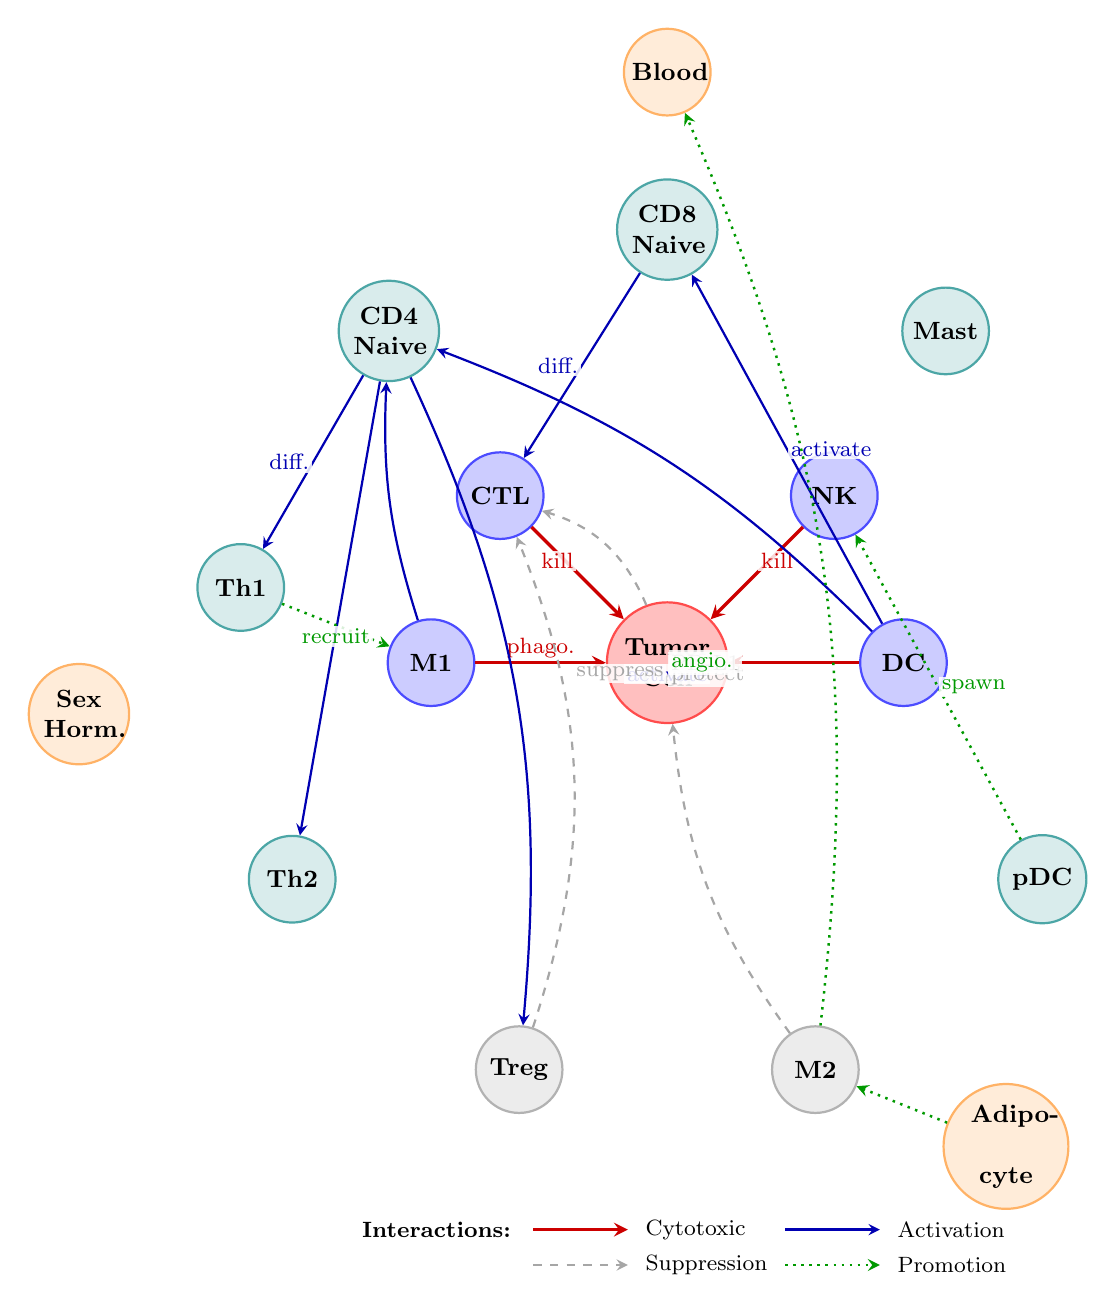
\begin{tikzpicture}[
  % Node styles
  agent/.style={circle, minimum size=1.1cm, text centered, font=\small, thick, inner sep=2pt},
  tumor/.style={agent, fill=red!25, draw=red!70, minimum size=1.4cm, text width=1.2cm},
  killer/.style={agent, fill=blue!20, draw=blue!70},
  adaptive/.style={agent, fill=teal!15, draw=teal!70, text width=0.9cm},
  regulatory/.style={agent, fill=gray!15, draw=gray!60},
  external/.style={agent, fill=orange!15, draw=orange!60, rounded corners=3pt, text width=0.9cm},
  % Edge styles
  cytotoxic/.style={->, >=stealth, red!80!black, line width=1.2pt},
  activation/.style={->, >=stealth, blue!70!black, line width=0.8pt},
  suppression/.style={->, >=stealth, gray!70, dashed, line width=0.8pt},
  promotion/.style={->, >=stealth, green!60!black, dotted, line width=0.9pt},
  % Label style
  lbl/.style={font=\footnotesize, fill=white, fill opacity=0.85, text opacity=1, inner sep=1pt},
]

% === CENTER: Tumor Cell ===
\node[tumor] (TC) at (0, 0) {\textbf{Tumor}\\\textbf{Cell}};

% === INNER RING (direct killers, r~3cm) ===
\node[killer] (CTL) at (135:3)  {\textbf{CTL}};
\node[killer] (NK)  at (45:3)   {\textbf{NK}};
\node[killer] (M1)  at (180:3)  {\textbf{M1}};
\node[killer] (DC)  at (0:3)    {\textbf{DC}};

% === OUTER RING (support/regulatory, r~5.5cm) ===
\node[adaptive]   (CD8N)  at (90:5.5)   {\textbf{CD8}\\\textbf{Naive}};
\node[adaptive]   (CD4N)  at (130:5.5)  {\textbf{CD4}\\\textbf{Naive}};
\node[adaptive]   (Th1)   at (170:5.5)  {\textbf{Th1}};
\node[adaptive]   (Th2)   at (210:5.5)  {\textbf{Th2}};
\node[regulatory] (Treg)  at (250:5.5)  {\textbf{Treg}};
\node[regulatory] (M2)    at (290:5.5)  {\textbf{M2}};
\node[adaptive]   (pDC)   at (330:5.5)  {\textbf{pDC}};
\node[adaptive]   (Mast)  at (50:5.5)   {\textbf{Mast}};

% === EXTERNAL (far out, r~7.5cm) ===
\node[external] (Blood)   at (90:7.5)   {\textbf{Blood}};
\node[external] (Hormone) at (185:7.5)  {\textbf{Sex}\\\textbf{Horm.}};
\node[external] (Adipo)   at (305:7.5)  {\textbf{Adipo-}\\\textbf{cyte}};

% ============================================================
% 1. CYTOTOXIC EDGES (red, solid, thick)
% ============================================================
\draw[cytotoxic] (CTL) -- (TC) node[lbl, midway, above left] {kill};
\draw[cytotoxic] (NK)  -- (TC) node[lbl, midway, above right] {kill};
\draw[cytotoxic] (M1)  -- (TC) node[lbl, midway, above] {phago.};
\draw[cytotoxic] (DC)  -- (TC);

% ============================================================
% 2. ACTIVATION / DIFFERENTIATION EDGES (blue, solid)
% ============================================================
\draw[activation] (DC)  -- (CD8N) node[lbl, midway, right] {activate};
\draw[activation] (DC)  to[bend right=12] (CD4N);
\draw[activation] (CD8N) -- (CTL) node[lbl, midway, left] {diff.};
\draw[activation] (CD4N) -- (Th1) node[lbl, midway, left] {diff.};
\draw[activation] (CD4N) -- (Th2);
\draw[activation] (CD4N) to[bend left=15] (Treg);
\draw[activation] (M1)  to[bend left=10] (CD4N) node[lbl, midway, below] {activate};

% ============================================================
% 3. SUPPRESSION EDGES (gray, dashed)
% ============================================================
\draw[suppression] (Treg) to[bend right=20] (CTL) node[lbl, midway, below left] {suppress};
\draw[suppression] (M2)   to[bend left=15] (TC)   node[lbl, midway, below right] {protect};
\draw[suppression] (TC)   to[bend right=25] (CTL)  node[lbl, pos=0.45, right] {PD-L1};

% ============================================================
% 4. PROMOTION EDGES (green, dotted)
% ============================================================
\draw[promotion] (Th1)  -- (M1)    node[lbl, midway, below] {recruit};
\draw[promotion] (pDC)  -- (NK)    node[lbl, midway, right] {spawn};
\draw[promotion] (M2)   to[bend right=15] (Blood) node[lbl, midway, right] {angio.};
\draw[promotion] (Adipo) -- (M2);

% ============================================================
% LEGEND (compact, bottom)
% ============================================================
\begin{scope}[yshift=-7.2cm, xshift=-0.5cm]
  \node[anchor=west, font=\footnotesize\bfseries] at (-3.5, 0) {Interactions:};
  % Cytotoxic
  \draw[cytotoxic] (-1.2, 0) -- (0, 0);
  \node[anchor=west, font=\footnotesize] at (0.1, 0) {Cytotoxic};
  % Activation
  \draw[activation] (2.0, 0) -- (3.2, 0);
  \node[anchor=west, font=\footnotesize] at (3.3, 0) {Activation};
  % Suppression
  \draw[suppression] (-1.2, -0.45) -- (0, -0.45);
  \node[anchor=west, font=\footnotesize] at (0.1, -0.45) {Suppression};
  % Promotion
  \draw[promotion] (2.0, -0.45) -- (3.2, -0.45);
  \node[anchor=west, font=\footnotesize] at (3.3, -0.45) {Promotion};
\end{scope}

\end{tikzpicture}